\chapter{Analysis of Twitter's Social Structure}


Stuff to add to this section:
\begin{itemize}
\item Change tweet features for each simulation and make comparison on these differences
\item Observe differences in patterns when network generation parameters are altered
\item Link up section to previous section (i.e. how did the previous research help and how does this build on that work?)
\item Explain how this section becomes the basis for work in 'main chapter 3'.
\item (e.g. Issues with current method (too long, requires network, inaccurate due to having to choose users with fewer followers), so need a quicker, more accessible and online approach).
\item Explain the Mechanical Turk questions in more detail, with examples.
\item Discuss about the machine learning approach used (logistic regression and how it works)
\item Link 'retweet volume' to 'retweet group size'
\end{itemize}


In the previous chapter, a series of studies were conducted into Twitter with respect to message propagation through retweeting. In particular, research was done to provide an understanding of the patterns produced through retweets and how their properties relate to the Twitter users that the Tweets pass through.

Of particular interest, however, is the social graph underlying Twitter, which describes how the users are interconnected and dictates the information flow between them. It has been discussed that users with a higher follower count are more likely to have their Tweets retweeted and that some users can have their Tweets forwarded through many hops indeed, so that information may be passed between different communities of users.

In addition to the effects of user influence,  several other factors also govern an individual retweet decision of a given user for a particular Tweet. These include properties of the Tweet, such as whether, or not, the Tweet contains a URL, whether it mentions a particular user, whether the user even has an opportunity to view the Tweet, and so on.\\
These factors account for the individual user's retweet decision and the almagamation of every user's retweet decision on the Tweet describes the Tweet's overall retweetability and, which determines how far the Tweet can propagate.

However, it is believed that the topology of the network, below the level of user influence, can play an important role in facilitating (or inhibiting) Tweet propagation by opening and closing available retweet pathways between users and groups of users.\\
Whilst retweet decisions based on Tweet features alone (such as the actual content of the Tweet or a URL the Tweet points to) may imply a level of interest in the Tweet, the influence of users has a very large impact on how many retweets a certain Tweet receives. Thus, abstracting the concepts away from user influence may help in discovering methods for inferring which information is interesting.

Twitter's social structure has previously been described as being built from users creating edges between themselves through the act of following. A followship defines the direction of travel of information from the follower to the friend, and this illustrates how users with many followers immediately have their Tweets made available to lots of users before any retweeting even takes place.\\
As more edges are constructed between users, then the global initial spread of Tweets is increased, and with the addition of retweets, this has an even bigger effect. Although other infleuncing factors have been mentioned earlier, such as the notion of a user's network awareness and of user influence, the organisation of users on the graph and the differences in observed propagation pattern is an interesting avenue for research towards uncovering interestingness.

In this chapter, various user network types are used to simulate retweet behaviour between users on Twitter. The behaviours are studied in order to research the propagation patterns observed in different network structure types. Non-realistic and realistic networks are used to highlight the low-level propagation in these networks and the similarities between more realistic simulated networks and Twitter's own social graph.\\
This research is then used to generate the methodology for estimating Tweet interestingness based on an \textit{expected} Tweet popularity, as is discussed further later in the chapter.


\section{Observing Differences in Propagation Patterns Between Different Network Structures}
In this section, simulations are carried out in three different network topologies - a path (or `linear') network, a random network, and a scale-free network. In the experiments, individual user \textit{decisions} are used as the bases for demonstrating Tweeting and retweeting.  

The simulation algorithm and ideas behind the model used for generating the simulated users' retweet decisions are adapted from the work carried out in \cite{zhu11} and \cite{peng11}, which introduces methodologies for illustrating Tweet spread through a given network of users.\\
From the analyses of the simulation experiments, of interest is whether, and how, changing the network structure does affect retweet propagation patterns, and whether a simulation can mimic Twitter's own bhevaiour in terms of retweet spread.

Measuring retweet behaviour is carried out through studying the distribution of retweet group sizes that result from running the experiments, as is described in later sections.


\subsection{Overview of the Simulation Algorithm}
The algorithm covers the simulation of Tweet propagation through a given set of connected users by emulating retweet decisions of each user who receives the Tweet. The retweet decision is made based on a logistic regression, as is described later.

\cite{zhu11} developed a simulation algorithm which carried this out, which was found to work accurately. This algorithm was modified to fit the purposes of the experiments in this section.\\
In essence, the simulation initially requires a graph of connected users, $U$, and a Tweet, $t$, to be retweeted between them. It begins by initialising a set of users, $S$, to contain the followers of a particular $u_s \in U$, which represents the user $\aut{t}{O}$. As such, users in $S$ are the current set of users to have $t$ on their home timeline.\\
The procedure then iterates over timesteps, at each stage checking the retweet probability of each $u \in S$. If $u$'s retweet probability is suffuciently great for $t$, then $u$ retweets $t$ by being removed from $S$ and then added to $\rt{t}$, which represents the set of users who have retweeted $t$. The followers of $u$ are then added to $S$.\\
A threshold value, $TH$, is used to emulate the idea of Tweet `decay'. The reasoning behind this is that as time goes by, more and more Tweets arrive onto the home timeline, pushing the previous Tweets further down, whether they are interesting or not. Tweets may be ignored and not retweeted if the user has not viewed their home timeline for a while or if the user decides the Tweet is not of a sufficient quality to retweet it. If a Tweet is pushed down to the extent that is out of view, or out of the current page, then the chance of that user retweeting that Tweet is reduced. Thus, if a user is in $S$ for more iterations than specified by $TH$, then the user is removed from $S$, meaning they cannot retweet the Tweet.\\
Users who have retweeted $t$, or are unable to do so (either by having previously retweeted it or by exceeding $TH$) are prevented from being (re-)added to $S$.

The algorithm terminates either when the timesteps exceed the maximum allowed, $T$, or when $S$ becomes empty. This results in the retweet group, $\rg{t}$, which comprises the final set, $\rt{t}$, along with the initial $u_s$. As in the previous chapter, $\rc{t} = |\rt{t}|$.

Therfore, the additional necessary components to run the simulation are the functionality to build the user graph, a constructed Tweet, and functionality for generating a retweet probability for each user who receives the Tweet.

\newfloat{algorithm}{H}{lop}
\begin{algorithm}
\caption{Simulation of retweet decisions in a given network of users}
\begin{algorithmic}[1]
\Procedure{simulate}{graph of users $U$, tweet $t$}
    \State $RT\gets$ empty set \Comment{To hold users who retweet $t$}
    \State $T\gets$ number of timesteps allowed
    \State $TH\gets$ maximum timesteps \Comment{Emulate $t$ `slipping' down timeline}
    \State $us\gets$ source User selected from $U$
    \State $S\gets$ initialise to followers of $us$
    \Statex % new line
    \ForAll{$ti$ in range $(0,T)$}
        \ForAll{$u \in S$}
            \State $P\gets$ retweet probability of $u$ on $t$ in range $(0,1)$
            \State $r\gets$ random number in range $(0,1)$
            \If{$P > r$}
                \State Remove $u$ from $S$
                \State Add $u$ to $RT$
                \State Add followers of $u$ to $S$
            \Else
                \State increment $u.\textrm{TIME\_HELD}$
                \If{$u.\textrm{TIME\_HELD} > TH$}
                    \State remove $u$ from $S$ \Comment{$u$ has held $t$ for too long in timeline}
                \EndIf
            \EndIf
        \EndFor
        \If{$|S| = 0$}
            \State return $RT$ \Comment{No more users can retweet $t$}
        \EndIf
    \EndFor
    \State return $RT$
\EndProcedure
\end{algorithmic}
%\caption{Algorithm to simulate retweet decisions in a given network of users.}
\label{algo1}
\end{algorithm}


\subsection{Generating a User's Retweet Probability} 
As prevoiusly mentioned, \cite{zhu11} used a predictive model for retweet decisions based on a logistic regression, which was demonstrated to be capable of accurately predicting a user's retweet chance on a given Tweet at a given time. The regression was trained on a set of user, tweet and context features in order to classify a likelihood on the binary decision: retweet or no retweet, such that if $P = 1$ then the retweet will definitely occur.


\subsubsection{Machine Learning}
Machine learning is the term given to the family of techniques that allow a program to make predictions for the outcome of unseen instances based on an observed and known history of occurrences. There are many types of machine learning classifiers that are suitable for different purposes, such as for predicting an expected outcome from a set of nominal categories, for predicting a value from a continuous range, or for predicting the \textit{probability} of a binary outcome.

Most machine learning techniques involve the training of a predictive model, which contains the information on known outcomes for a set of features. The model is then used to estimate an unknown outcome, usually with a probability on the \textit{confidence} of the classification, for new sets of instances.

For example, consider three attribute variables, $A$, $B$, and $C$, each of which can be equal to one of two nominal values; \textsc{True} or \textsc{False}. A particular machine learning algorithm trains a model based on its knowledge that;
\begin{itemize}
    \item $A\gets$ \textsc{True}, $B\gets$ \textsc{False} $\Longrightarrow$ $C\gets$ \textsc{True}
    \item $A\gets$ \textsc{False}, $B\gets$ \textsc{False} $\Longrightarrow$ $C\gets$ \textsc{False}
\end{itemize}
Although training of predictive models nearly always involves using more than two instances, the history of these example instances indicate that $C$ is more strongly associated with $A$ than with $B$. As more instances are added showing similar behaviours, then the association becomes stronger, to the extent that the technique will predict $C\gets$ \textsc{True} in instances where $A\gets$ \textsc{True} (and vice versa) with higher confidence.

In this case, $A$, $B$, and $C$ are known as the `features', and a set of such features form the `instance'. Once a trained model has been constructed, the machine learning algorithm will only be able to make predictions using instance features it has knowledge of. For example, if the example technique was now given an instance containing a feature $D$, then the example technique will not know how changes in $D$ will affect $C$'s outcome.

If there is not a strong correlation between the features in a dataset, then the confidence on classification of a particular feature will be weaker. Although this example has focussed on boolean (nominal) data types, many machine learning classifiers are able to work with features that are higher dimensional nominal values, contunuous reals, and so on, and will apply weights to the different features based on their level of influence to other features in the instance.


\subsubsection{The Logistic Regression}
Logistic regression analysis can be used as a machine learning technique for working with binary outcomes based on a set of predictor variables (or features) \cite{hosmer13}, which makes it an appropriate approach for predicting the binary retweet decision. As mentioned previously, logistic regressions have been frequently used in retweet analysis \cite{castillo11} \cite{zhu11} \cite{peng11} \cite{naveed11} \cite{hong11}.

An implementation of the logistic regression algorithm was written in the Python programming language, which formed the basis of calculating the value for $P$ mentioned in the algorithm overview earlier based on a set of feautures of the Tweet and author user.


\subsection{Summary of Training Features}
\cite{zhu11} used the approach in order to accurately model retweet decisions in Twitter. A set of around 50 different features were used to train the logistic regression, with the retweet outcome (\textsc{True} or \textsc{False}) being the predicted classification in each case. These features included tweet-related features (such as content analysis, inclusion of URLs, etc.), and network and user features (followships, mentions, etc.).

Since the network structures themselves, and the propagation \textit{patterns}, are what are of interest in this section, the simulation is significantly simplified by using far fewer features, yet which are features that have been shown to have a strong influence on the retweet decision. As long as a consistent set of feature groups and values are used, the properties of the retweet groups observed should demonstrate the varying behaviours across the different user structures.

As such, each instance comprised the following four features associated with each Tweet, $t$, and where $u$ is the user currently making the retweet decision, \textsc{retweet};

\begin{table}[h]\footnotesize
\begin{center}
\begin{tabular}{ l | c | l }
	Feature & Data type & Description\\
	\hline
	\hline 
	\textsc{follows}    & \{\textsc{True, False}\} & \textsc{True} if $u \in \fos{aut{t}{O}}$\\
    \textsc{followed}   & \{\textsc{True, False}\} & \textsc{True} if $u \in \frs{aut{t}{O}}$\\
    \textsc{mentioned}  & \{\textsc{True, False}\} & \textsc{True} if $u$ is mentioned in $t$'s content\\
    \textsc{url}        & \{\textsc{True, False}\} & \textsc{True} if \texttt{http://} or \texttt{https://} in $t$'s content\\
    \hline 
    \textsc{retweet}    & \{\textsc{True, False}\} & \textsc{True} if $u \in \rt{t}$\\ 
    \hline
\end{tabular}
\end{center}
\caption{Training features for the logistic regression.}
\label{table:logisticregressionfeatures}
\end{table}

The \textsc{url} feature has, in the literature, often been found as a large impacting feature on retweets in Twitter, especially in \cite{alonso10}, who use it as their basis for determining which Tweets are interesting.


\subsection{Training the Model}
In order to train the logistic regression model, data was required from Twitter so that the instance sets of features could be built. 

Data collection for these experiments again utilised Twitter's REST API, which was queried between March and June 2012 to collect a set of around 12,000 Tweets and retweets. Since this time was before the mandatory switch-over to v1.1 of the REST API, the public timeline could again be used to collect the data without the necessity of crawling through the social graph.\\
In this case, it was particularly necessary that non-retweets were also collected in order to provide the negative case when training the regression model, so that there were instances where the \textsc{retweet} feature could be \textsc{False}.

In cases where the collected Tweet was a retweet, further calls were made to the API to determine the relationships between the retweet's author and the original Tweet's author in order to satisfy the required \textsc{follows} and \textsc{followed} features.
Where the collected Tweet was not an instance of retweet, there is no original author to examine the relationships between. In these cases, further Tweets were retrieved for the user in order to find their retweet rate in terms of the ratio of retweets to Tweets on their user timeline and an analysis of the relationship between these and the original authors. This was used in conjunction with the user's follower and friend count to determine a probability of the `faux' followships.

After storage, the regression model was trained using features extracted from the raw data, which the simulation algorithm could then use to generate the required retweet probability, $P$.


\subsection{Running the Simulations}
Once the model had been trained, the simulations could be run. In each simulation experiment, a network of users was generated, as described in the next section, and a Tweet object was created.\\
This Tweet object contained information on whether or not it contained a URL and if it mentioned one of the users in the generated network. 

Various parameters - such as the $TH$, the size of the user network, $U$ to be generated, $t$'s particular parameter for the simulation, and any weightings on the decision probability prediction generator - could be altered to affect the strength or correlation of the patterns produced by the different network structure types.


\subsection{Network Analyses}
In this section, three network structures are assessed in terms of the differences in the patterns of propagation each expresses. Each generated graph is a \textit{directed} graph in order to illustrate the followships between the user nodes, and to support the use of the \textsc{follows} and \textsc{followed} features required in the decision probability calculation.

In each case, the same set of generated Tweets were used, but different structures required the various parameters to be set slightly differently. As such, each network structure will present with different proportionate retweet group size distributions; of interest to this work is the difference in \textit{pattern} of the distribution.


\subsubsection{Path Network}
The first assessed structure was to illustrate the pattern on a non-realistic social network structure; a path network.

Path networks are one of the simplest type of graph, and a linear directional path network consists of the graph of users, $U$, of size $n$, in which each user $U_i \forall 0 \leq i < n$ is followed by user $U_{i+1}$. As a result, each $u \in U$ has precisely one follower and one friend, except the users $U_n$ and $U_1$ respectively.\\
$n$ is the only parameter necessary in the construction of this user graph.

\begin{figure}[h]
\centering
\includegraphics[scale=0.8]{4.Chapter2/Media/path_network.png} 
\caption{Example of a path network.}
\label{fig:path_network}
\end{figure}

In this graph, the size of the retweet group is, by definition, equal to the depth of penetration, as there is only one path (or retweet chain) available for propagation to occur down. As such, in each case, the retweet tree representing a resultant retweet group formed in this type of network will have the same structure as the graph itself, yet with a size dependent on the collective retweet decisions of the users.

Since each internal user has only one follower, the likelihood of a retweet decision being positive at each timestep is somewhat progressively reduced, and thus is much more likely to tail off sooner than in graphs with more propagation avenues. This is also due to the fact that each retweet can only reach an audience of size 1 at each time step, and thus the survival of the retweet cannot rely on a summation of many users' retweet decisions. 

\begin{figure}[h]
\centering
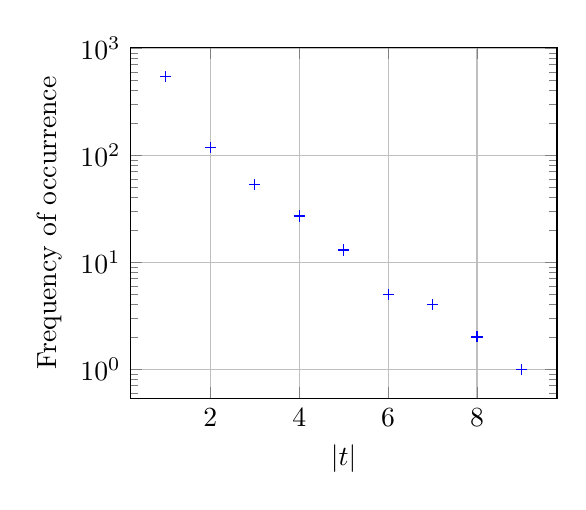
\begin{tikzpicture}
 \begin{semilogyaxis}[
        xlabel=$|\rg{t}|$,
        ylabel=Frequency of occurrence,
        width=7cm,
        grid = major]
    \addplot[only marks,mark=+,blue] plot coordinates {
        (1,540)  (2,118)  (3,53) (4,27) (5,13) (6,5) (7,4) (8,2) (9,1) (10,0)
    };
\end{semilogyaxis}
\end{tikzpicture}
\caption{Frequency distribution of retweet group sizes in path network simulations}
\label{fig:linear}
\end{figure}

The likelihood of a particular user achieving the opportunity to receive the Tweet, in order to then retweet it, becomes the product of the probability function the further it travels through the graph, in which user $U_i$ requires each user from $U_{i-1}$ to first make a positive retweet decision. For example, if each user has probability $p$ of retweeting the Tweet, then each user's chance of retweeting the Tweet is $\frac{1}{p^i}$, where $i$ is the position of the user in the graph.

Therefore, as might be expected, the frequency distribution of retweet group sizes shows a half-life type behaviour demonstrating a logarithmic pattern with many small retweet groups followed by a series of exponentially smaller groups.\\
This user structure illustrates well how some users that might find the Tweet interesting, and who may decide to retweet it, do not even get the chance to view it in order to make the decision. Although this is accentuated in this structure, the same principle applies to any non-complete social graph, and demonstrates how the way users are connected can have a large impact on the retweetability of a particular Tweet.


\subsubsection{Random Network}

\begin{figure}[h]
\centering
\includegraphics[scale=0.8]{4.Chapter2/Media/random_network.png} 
\caption{Example of a random network where $n = 5$ and $p \sim 0.5$.}
\label{fig:path_network}
\end{figure}


The random network was the next user structure to be analysed. Although it is certainly more similar to a real-life social graph than a path network, it is much more basic and uniform and does not consider user communities and clusters or different levels of influence in users in terms of their follower and friend counts.

A random social network is defined as the case in which the graph of user nodes, $U$, and where $n = |U|$, consists of each user, $u$, having probability $p$ of following each other $u_i \in U \forall 0 \leq i \leq n$ and where $u_i \neq u$. Thus, as $p$ is increased, then the likelihood of $u$ following a $u_i$ increases, causing the overall network edge density to increase. In general, therefore, the average number of followers and friends of a user is proportional to $p.n$.\\
The only parameters needed for constructing such a graph are $n$ and $p$.

\begin{figure}[h]
\centering
\begin{tikzpicture}
 \begin{semilogyaxis}[
        xlabel=$|\rg{t}|$,
        ylabel=Frequency of occurrence,
        width=7cm,
        grid = major]
    \addplot[only marks,mark=+,blue]
       file {4.Chapter2/data/random.dat};    
\end{semilogyaxis}
\end{tikzpicture}
\caption{Frequency distribution of retweet group sizes in random network simulations}
\label{fig:random}
\end{figure}

The frequency distribution demonstrates a very large proportion of mid-range values for $\rg{t}$, indicating that Tweets tend to have a consistent spread amongst the network, as might be expected. There are few smaller groups since there are no users that have disproportionately smaller spheres of influence, and each user has many incoming edges and a proportionately similar number of outgoing edges. As such, there are more mid-range retweet group sizes than smaller ones.\\
However, as in any distribution so far examined, the distribution of retweet group sizes must eventually tail off due to the natural eventual reduction in retweet decisions being successfully made as retweet chains increase in length.


\subsubsection{Scale-Free Network}
The final network structure examined in this section is the scale-free network. Also known as `small world', scale-free graphs are generally throught to be representative of the general structure of online social networks \cite{mislove07} and, indeed, they are used to describe the interconnections of real-world properties, such as friendship groups and food webs \cite{guido07} \cite{hein06}.\\
Essentially, scale-free networks dictate that there are a small number of nodes with a high degree and many nodes with a low degree and are usually generated through some form of preferential attachment algorithm. Thus, this type of network supports the notions of user communities and influential users in terms of those demonstrating a disproportionately large follower count. The other user structures studied do not have the scope for emulating this property of interconnection between the user nodes.

Scale-free networks are constructed such that the distribution of the degree of the graph's nodes follow a power-law-type distribution in that the distribution of this degree is lograthimic. \\
For these analyses, NetworkX\footnote{http://networkx.lanl.gov}, a Python graph and networking package, was used to generate directed scale-free graphs of users, which essentially accepts a network size, $n$, and edge density $d$ as the graph construction parameters. 

\begin{figure}[h]
\centering
\begin{tikzpicture}
 \begin{loglogaxis}[
        xlabel=$|\rg{t}|$,
        ylabel=Frequency of occurrence,
        grid = major,
        width = 7cm,
        legend entries={Twitter data, Generated scale-free data}]
    \addplot[only marks,mark=*,red]
       file {4.Chapter2/data/comparison-real.dat};
    \addplot[only marks,mark=*,blue]
       file {4.Chapter2/data/comparison-scale-free.dat};
\end{loglogaxis}
\end{tikzpicture}
\caption{Comparing the retweet volumes distribution from scale-free graph simulation to data from Twitter's graph}
\label{fig:real-scalefree}
\end{figure}

From simulations of the algorithm through these scale-free networks, a logarithmic trend is observed similar to that demonstrated from the `real' Twitter data analysed in the previous chapter and published in \cite{webberley11}, and the similarities in the distribution pattern is illustrated by Figure \ref{fig:real-scalefree}.


\subsection{General Comparison of Propagation Characteristics across Different Graph Structures}
In this section, three different network structures have been compared, and whilst the path network is very unrealistic in terms of a representation of a social network, the differences in propagation behaviour presented by each do show how the interconnection of users on the graph can have a large effect on the spread of a Tweet. A small set of features to govern retweet features were used in order to accentuate the difference made by the user structures themseleves.

This has demonstrated that, in addition to the processes behind a user's individual retweet decision, the eventual spread of a Tweet also depends somewhat on how the original author's local network is arranged. Thus, the retweet decision of each involved user along with the available information pathways provided by the underlying social structure both contribute to the overall retweetability of a Tweet. 

If there are many edges in the network, such as in the case of the random network, then there are many more routes for peopagation to occur down to and from each user, due to the relatively large in- and out-degree of each user node on the graph. This increases the number of users who end up receiving the Tweet and then have the chance to make a retweet decision. This resulted in there being a larger distribution of larger retweet group sizes than smaller ones, before naturally diminishing again. Despite this high throughput of retweets, which provides a high level of information \textit{recall} for the users, the random graph structure is likely to demonstrate a low \textit{precision} in terms of the interestingness of the received Tweets.\\
This is due to the large number of users having the opportunity to retweet the Tweet, increasing the chance that the `noisy' information will be filtered through.

The path network demonstrated very poor propagation, and required that its simulation parameters were altered to facilitate retweet behaviour significantly more than in the other graph structures in order to produce any observable pattern. The results showed that propagation down a single allowed chain cannot be an effective way to spread Tweets, as it required each user in the chain to retweet it so that the successive users can have a chance to view it.

Whilst the scale-free network does not have the same general propagation throughput as the random network, it does demonstrate retweet patterns similar to those observed in data from Twitter's own social graph. This complements the findings of \cite{mislove07} and \cite{hein06} in terms of online social networks emulating real-life social networks having scale-free properties.\\
This type of structure supports areas of the graph with denser communities, as is shown to exist by \cite{java07}, and have the potential for facilitating very large numbers of retweets if influencial users are involved, but illustrate how Tweets `travelling' through less dense areas (and less-influencial) users will not be as demonstrably popular.



\section{Using the Social Graph as a Method for Inferring Interestingness}
The graph analyses in the previous section have demonstrated a method for generating a $\rg{t}$ for a given Tweet, $t$. Since $\rc{t} = |\rg{t}| - 1$, then the simulation algorithm used can be used to estimate a retweet count for a given Tweet. Although it has been discussed that although an individual's retweet decision does generally imply that user's interest in the Tweet, the overall retweet count of a Tweet is capable of denoting that Tweet's popularity. However, this value could be used in tandem with the expected estimated retweet count of a Tweet in order to determine if the Tweet is, in fact, interesting.

This notion is based on the idea that if a Tweet is more popular than expected, then there is something about that Tweet that makes it more \textit{interesting} than similar Tweets that are less popular, such as some breaking news or a link to a controversial article.\\
For example, consider the case of two Tweets, written by the same author, and both containing the same instances of feature values, such as the inclusion of a URL or a mention. If one of these Tweets achieves significantly more retweets than the other, then there must be some non-trivial feature of the more popular Tweet that makes it stand out to the audience, and thus allows it to be perceived as more \textit{interesting}. This is because the features taken into account are very static, and do not take into account any depth of the actual content of the Tweet.\\
Similarly, if most Tweets of a user achieve between one and two retweets, then the expected retweet count for this user's future Tweets is likely to be similar. If, however, the author posts a Tweet which achieves an observed total of 10 retweets, then this is more than what was expected. If a Tweet achieves one or zero retweets, then this is as expected or less than expected, and is therefore not interesting.

As such, a method is proposed based on the following two points;
\begin{itemize}
    \item observed $\rc{t} >$ expected $\rc{t} \Longrightarrow t$ is interesting
    \item observed $\rc{t} \leq$ expected $\rc{t} \Longrightarrow t$ is non-interesting
\end{itemize}

Although it was found, in the previous chapter and in other relevant literature, that pseudo-generated scale-free networks can be representative of Twitter's own social structure, a user's actual own local social network would more accurately portray the links between the users surrounding the original author of a Tweet. By constructing a network based on a user's own local network, then the method would effectively be simulating the Tweets' propagation through the edges representing the followships of the actual users in Twitter's social graph.

Thus, in the simulation algorithm, the user in question is $u_s$, and the intiial value of $S = \fos{u}$. At each timestep, each user in $S$ would have the opportunity to retweet the Tweet, and therefore, by running the simulation, an estimation on the \textit{expected} value for $\rg{t}$ can be obtained, where $\aut{t}{O} = u_s$.\\
In particular, this method follows these steps;
\begin{enumerate}
    \item Select a user
    \item Collect that user's local follower network 
    \item Collect a set of that user's recent Tweets
    \item Construct a network based on the users and edges in the collected network
    \item Simulate the collected Tweets through the constructed network using the simulation algorithm
\end{enumerate}

This procedure would provide an estimated retweet group size for each Tweet, which could then be compared to the actual observed retweet count of the Tweet on Twitter.


\subsection{Data Collection}
Due to the scaling properties of breadth-first traversal of Twitter's social graph, it became infeasible to collect a user's local network containing users more than two edge `hops' away from the source user under the rate limitations of Twitter's REST API.\\
As mentioned, v1 of the REST API allowed 350 calls to the API each hour for each authenticated Twitter account. One call, for example, was required to obtain a list of up to 5,000 IDs representing the follower users of a particular user - the users one hop from the source user. An additional call would then be required to collect each of these user's own followers in order to provide the 2-hop representation of the local network from the source user.

For a user with a follower count of 700, a total of 701 API calls would be required to collect the user's local network within two hops - the one to retrieve the source user's immediate followers, and then one further call for each of the 700 followers. This would take over two hours of collection as it is, and to collect the third hop would require another exponential number of API calls.\\
If each of the 700 followers of the source user has, on average, 200 followers, then this would require  a further $700 \times 200 = 140,000$ API calls, which, in total, equates to over 402 hours of data collection time. Although some follower overlap is likely to be present among the users two hops away, when one considers that this is simply the time taken to collect the local network for one user, then it becomes clear that this must still be an impractical approach.

In the previous chapter it was found that the vast majority of retweets do actually occur \textit{within} two hops of the source user, in that retweet groups produced have a maximum path-length of less than three. In addition, as mentioned, online social networks are `closer' than real-life social networks, and was found to have a value of around four degrees of separation in Facebook. These points help to justify the decision made to class a user's local network as those users and edges existing within two hops from the source user.

In June 2012, the Twitter REST API was used in order to conduct a random walk through Twitter's social graph. Starting at selecting an initial user, an edge expressing the followship of a random follower was chosen in order to select the next user. This continued for each of the selected users in turn and, for each user selected, the most recent 300 Tweets and surrounding information was collected along with that user's local follower network within two hops. The friend network (i.e. the outward edges from each user) was ignored, as only the directional outward flow of information from the source user was useful in this experiment.\\
If, at any stage, the currently selected user did not have any followers, the collection algorithm backtraced to the previous user and another follower was selected instead. The crawler continued until the rate limit for the current request window was met, at which time the current data state was stored, and then waited until the rate-limit was reset before continuing.

The data collection resulted in a set of 33 Twitter users, each with a full local network collected and a set of up to 300 Tweets. In total, around 10,000 Tweets were collected in order to carry out the simulations. It was decided that the previously trained regression model would be re-used as part of the retweet decision engine in this experiment also, and so no further training data was required for collection.



\subsection{Validating Results}



Needed to validate results using human input. Machines themselves are generally unable to express human interests, so results need to be properly evaluated.

\subsubsection{Crowdsourcing}
Discuss crowdsourcing, its uses, how it is useful in this area. Talk about its history (with any references), and then about mechanical turk.
\\
Mention mechanics of mechanical turk, how it is US only (but we used crowdflower - which autmatically handles submission to MT and several other crowd-sourcing services.

\subsubsection{What We Wanted to Assess}
Used MK, etc.

\subsubsection{Constructing the Questions}
Set up questions (i.e. 5 tweets - choose most interesting and least interesting), give example of this.


In order to validate our prediction results, we ran a pilot user study in order to obtain some human input on the interestingness of each tweet. We compiled the tweet data into a set of questions which were submitted to Amazon's Mechanical Turk. Each question consisted of five tweets from our dataset and each Mechanical Turk Worker (MTW) undertook five questions. Each question asked the MTWs to select which tweet was the most interesting of the five, and which was the least interesting.
\\
For consistency we ensured that at least three MTWs had answered each question. When selecting tweets to include in the Mechanical Turk questions, we excluded those which are `@-replies' - i.e. tweets which begin with another user's screen-name and typically form part of a conversation between two or more users. This meant that there were around 4,500 tweets in total in the questions.

Through using the model and simulating each user's tweets through their individual local networks we achieved around 86\% accuracy in correctly predicting the number of times each tweet was retweeted. 
\\
The precision in predicting the \textit{interestingness} of each tweet was around 30\%. While this value is low, it does mean that in 30\% of cases, a tweet that we predicted to be interesting was verified to be interesting by at least three MTWs all selecting one tweet from a set of five. In addition, when simulating the questions by randomly choosing the most `interesting' tweet of the five in each case, the performance was unable to near our precision even after several thousand iterations.

\subsection{Improving This}
idea is there - need better idea for getting expected retweet value! problem is two-fold, but related - need too much data, and can only evaluate users with sparser local networks.
\\
Need offline methodology.
\\
One route for this would be to try and infer a user's local network from a set of their immediate parameters, drawing on our earlier work suggesting that the Twitter network has the properties of a scale-free small-world graph. Through studying graph patterns, it is possible to make sensible inferences on the edges and nodes of a user's local network based on their follower count. From this, a graph edge density can be calculated, $ d = \frac{|E|}{|N|(|N|-1)} $, for use in generating a scale-free network.
\\
Since, for these preliminary experiments, we were only able to collect data from users with a more modest local network, the real and predicted retweet values were both relatively low, allowing more room for error. When simulating much larger local networks involving many more real retweets for each tweet, predicting interestingness, with some threshold value, may become more accurate and thus help improve the precision. The reason for this is that the retweet count of tweets that naturally get retweeted many tens, hundreds, or more times is likely to vary more with interestingness than those that are naturally only retweeted very few times.

\section{Future Work}
There is much further research that could be carried out based on the results in this chapter. Now that the foundation has been laid for simple retweet prediction based on network analysis, research could begin to look at ways in which, as mentioned, networks could be generated based on a few environmental features surrounding users.
\\
This would allow for quick generation of user networks (bypassing the need for data collection) and would also support the same calculations for more highly influential users (users with more followers and more retweets per Tweet).
\\ \\
For this research, the notion of the network will continue and form the basis of the environmental features in the next chapter. Since we now know that the network plays an important role in dictating the way in which information can propagate

\section{Summary}
In this chapter we aimed to carry out a study on the behaviour of propagation through different types of social graph structures and to introduce our ongoing work into predicting the interestingness of tweets from their retweet patterns.
\\
Using a set of tweet and user features, we trained a regression model which we used to simulate a number of tweets through different network types. We produced a distribution of retweet volumes for each network type and confirmed that, with the same tweet features, different network configurations do indeed facilitate different retweet behaviours in terms of propagation spread. We were also able to compare our results to data from Twitter to verify that Twitter's own social graph most closely resembles a scale-free small world graph.
\\
We then finished by discussing how we used the trained model to simulate real networks from Twitter, along with the tweets that were passed through these networks, in order to try to predict how interesting a tweet is based on its retweet patterns. While we were able to often correctly predict the retweet outcome of a tweet, we found that more work would be required to improve the performance of predicting whether or not these tweets are truly interesting to users.
